% Test tex file!

\documentclass[a4paper,12pt]{article}
\usepackage{times}  % DO NOT CHANGE THIS
\usepackage{helvet} % DO NOT CHANGE THIS
\usepackage{courier}  % DO NOT CHANGE THIS
\usepackage[hyphens]{url}  % DO NOT CHANGE THIS
\usepackage{graphicx} % DO NOT CHANGE THIS
\urlstyle{rm} % DO NOT CHANGE THIS
\def\UrlFont{\rm}  % DO NOT CHANGE THIS
\usepackage{natbib}  % DO NOT CHANGE THIS AND DO NOT ADD ANY OPTIONS TO IT
\usepackage{caption} % DO NOT CHANGE THIS AND DO NOT ADD ANY OPTIONS TO IT
\frenchspacing  % DO NOT CHANGE THIS
\setlength{\pdfpagewidth}{8.5in}  % DO NOT CHANGE THIS
\setlength{\pdfpageheight}{11in}  % DO NOT CHANGE THIS
\usepackage{algorithm} %format of the algorithm 
\usepackage{algorithmic} %format of the algorithm 
\usepackage{multirow} %multirow for format of table 
\usepackage{amsmath} 
\usepackage{xcolor}
\usepackage{amssymb}
\usepackage{amsmath}
\usepackage{CJKutf8}
\usepackage{courier}
\usepackage{booktabs}


\begin{document}
\begin{CJK}{UTF8}{gbsn}
% \begin{CJK}{UTF8}{gkai}

\title{强化学习:作业一}

\author{傅浩敏 MG20370012}

\date{2020年10月19日}

\maketitle

\section{作业内容}
在“蒙特祖马的复仇”环境中实现Dagger算法。

\section{实现过程}
首先在 \texttt{model.py} 中创建自己的模型。我实现了CNN和KNN两个模型,需要注意的是KNN模型会采用随机的策略生成第一批动作。由于神经网络模型效果不够明显,因此在后续实验中均采用KNN模型。不过我依然保留了卷积神经网络模型的代码以供参考。然后我们需要在 \texttt{Dagger.py}中实例化选择的模型对象并实现 \texttt{update} 和 \texttt{select\_action} 方法。为了减小问题规模,我对默认参数进行了如下修改:\\\\
\centerline{\texttt{--num-steps=50 --test-steps=200}}
\centerline{\texttt{--num-frames=4500 --log-interval=5}}\\\\
之后修改 \texttt{main.py} 中的代码,实现数据标注代码。为了更够增量式地进行实验,我将历史图片和标签数据保存在 \texttt{data} 文件夹下,在 \texttt{config.ini} 中记录了当前训练的轮次,在 \texttt{performance.txt} 中保存了历史实验数据。最后,在主文件夹下运行 \texttt{python main.py},在图片窗口中输入对应的标签,在4500个样本标注完成后程序运行结束。标签含义如下:\\
\begin{table}[H]
	\begin{tabular}{@{}ccccccccc@{}}
		\toprule
		0    & 1  & 2  & 3  & 4  & 5  & 6   & 7   & 8    \\ \midrule
		原地不动 & 跳跃 & 向上 & 向右 & 向左 & 向下 & 向右跳 & 向左跳 & 随机动作 \\ \bottomrule
	\end{tabular}
\end{table}
\section{复现方式}
可以在修改 \texttt{--num-frames} 参数后,在主文件夹下运行 \texttt{python main.py} 继续实验。也可以配置 \texttt{config.ini} 中的 \texttt{data\_index=0} 并在主文件夹下运行 \texttt{python main.py} 来重新开始实验。
\section{实验效果}
见图 \ref{performance}。累计奖励随样本训练量的增加而增加,并逐渐趋于稳定。访问专家的次数随样本训练量增加而线性增加\footnote{在原始代码中 \texttt{query\_cnt} 始终为0,为了满足实验结果的合理性,我将数据标注轮次作为访问专家的次数。}。
\begin{figure}[h!]
\centering
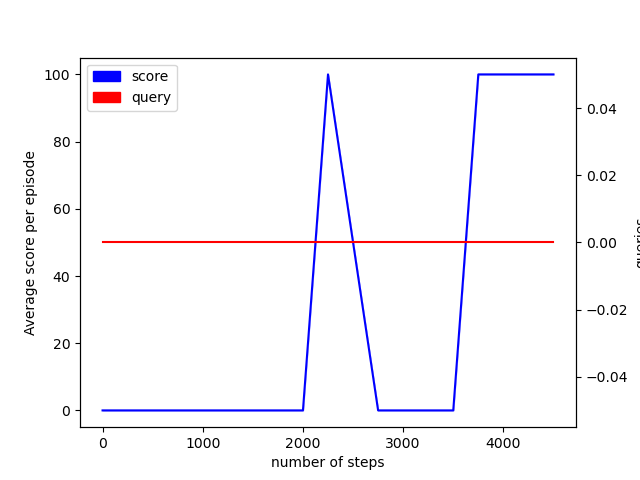
\includegraphics[width=8cm,height=7cm]{./code/performance.png}
\caption{Dagger算法}
\label{performance}
\end{figure}
\section{小结}
在这次实验中,我发现Dagger算法需要频繁访问专家,因此在训练模型时需要花费专家的大量时间和精力进行数据标注,训练成本极高,适用场景有限。在使用Dagger算法解决“蒙特祖马的复仇”时,我标注了4500张图片才能勉强稳定的吃到第一个钥匙,并且随着样本数据的增加,模型训练时间也会逐步增加,因此我们需要一个效率更高的学习方法。
\section{思考题}
在玩游戏的过程中标注数据时,我们只需要关注移动路径上的动作,而在Dagger算法中,我们需要标注模型在环境中探索产生的数据。使用游戏过程中标注的数据意味着模型直接学习专家路径,而Dagger算法则是在探索环境的过程中逐渐学习专家路径。这使得Dagger算法能够应对更加复杂的环境,但同时也需要更多的专家数据支持。

\end{CJK}
\end{document}